% begin module composition-functions
\begin{frame}
\begin{definition}[Composition of $f$ and $g$]
If $f$ and $g$ are two functions, then the composition of $f$ and $g$ is written $f\circ g$ and is defined by the formula
\[
(f\circ g)(x) = f(g(x)).
\]
\end{definition}

Imagine $f$ and $g$ as machines taking some input and producing some output. Then $f\circ g$ corresponds to attaching both machines end-to-end so that the output of $g$ becomes the input of $f$.

\psset{xunit=0.75cm, yunit=0.75cm}
\begin{pspicture}(-4, -2.5)(13,2.5) 
\footnotesize
\rput[r] (-3.1, 0){$x$}
\psline[linewidth=3pt]{->}(-3,0)(-2.25,0)

\rput(0.25,0){
\psMachine{$g$}{blue}
}
\rput (4, 0){$g(x)$}
\psline[linewidth=3pt]{->}(2.75,0)(3.5,0)
\psline[linewidth=3pt]{->}(4.5,0)(5.25,0)
\rput(7.75,0){
\psMachine{$f$}{red}
}
\rput (11.75, 0){$f(g(x))$}
\psline[linewidth=3pt]{->}(10.25,0)(11,0)
\end{pspicture} 
%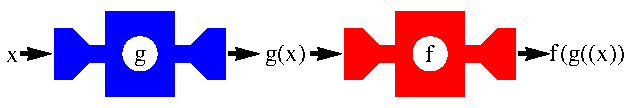
\includegraphics[height=2cm]{precalculus/pictures/01-03-machines.pdf}%

\uncover<2->{
The domain of $f\circ g$ is the set of all numbers $x$ in the domain of $g$ such that $g(x)$ is in the domain of $f$.  If the domain of $f$ is $A$ and the domain of $g$ is $B$, we write this as
\[
\{ x\in B |\ g(x) \in A\} .
\]
}
\end{frame}
% end module composition-functions